% !TEX root = ../../thesis.tex

\chapter{Discussions} % (fold)


Ce qui est chaud c'est d'avoir un pied dans la recherche et un pied dans les applications generale. Typiquement on veut faire passer des notions avancés comme le design of emergence et le role de la morphology. Des gens non initiés peuvent comprendre ce genre de chose mais ça demande beaucoup de mediation.


Faire des robots imprimés en 3D MIT

Nouvelle methodes de design et Explorer le role du corps


Evolution scientifique + open source

Evolution commune entre la science et la société (Fablab, internet of things)

Finalement qu'est ce que Poppy ?

Communauté/benchmark/foret de poppy/demonstrateur technologique

Education/art/importance du beta test

Nouvelle techno plus modulaire










printing:
\url{http://www.technologyreview.com/news/514071/wanted-a-print-button-for-3-d-objects/}



\section{Arduino} % (fold)
\label{sec:arduino}


DAVID Cuartielles: Arduino is an electronics prototyping platform that is used, by many, as a way to learn about digital electronics. It offers easy access to a whole body of knowledge. One of the key aspects of this technology is that, from the beginning, it was designed having the users in mind. It was made thinking that students would either buy a board or build their own, and that the system would offer a software abstraction good enough to enable them to quickly learn about embedded programming. Arduino includes the hardware and the software to get it to work, and the documentation to learn how to make it. The whole technology is open source. As a matter of fact, the Arduino project has become a reference project when talking about making open hardware available for others to use.

Arduino is used by students coming from almost every discipline at university level. Art and design students were our initial user group from, but by making the system easy to use to them, we made it easy for everybody. Many design studios, but also research groups, started using Arduino technology for its ease of use, as it makes things that should be easy to solve, easy to solve

% section arduino (end)

\section{TODO} % (fold)

mettre en place des outils de partage pour récuperer les travaux


Creer un board de descision autour du projet qui n'est pas constitué que de membre de l'équipe flowers.
Flowers appartient à certains courant de pensé en recherche et notre vision biaise de manière inconsciente le developpement du projet. Un projet robotique open source devrait justement permettre à different courant de travailler ensemble, de partager et surtout comparer les resultats. Le fait que Poppy soit né dans l'un et qu'on est les pleins pouvoirs dessus peut être consideré comme un problème pour des chercheurs d'autres courants qui par consequent vont preferer créer une autre solution non-compatible. On se retrouverai alors avec les mêmes problèmes de partage des resultats et de transfert entre labo.

De même la communauté devrait être geré par un consortium scientifiquo-educatif et non uniquement par nous.

Ces evolutions semblent importantes mais faite trop vite peuvent aussi nuire au projet car nous imposons une dynamique. A nous de preparer les choses pour transferer les choses au bon moment.


\section{Intro} % (fold)
La diffusion scientific comme on la propose necessite de faire de ce limiter à des composants classiques afin de favoriser leur disponilité. On peut penser que c'est un frein à l'innovation dans le sens où on utilise des composants existant plutôt que d'en créer de nouveaux. C'est vrai ...
Cependant, on peut imaginer un certain nombre de cas ou c'est possible d'innover tout en laissant la possibilité de diffuser. On pourrait imaginer qu'un robot humanoide et d'une grande complexité donc difficle sans tout changer. Pourtant il ne s'agit que de choisir les bonnes technos qui sont scalables. Preferer l'impression 3D ou le decoupage laser à l'usinage classique, utiliser arduino plutôt qu'une electronique perso.

Dans le cas d'electronique custom et plus complex que ce que permet arduino, il existe des sites comme Circuit hub qui permettent d'industrialiser automatiquement, les gens pouvant directement acheter chez eux. Pareil pour la méca, on peut avoir des boutiques en lignes poru diffuser les pièces.

Les assemblages mécanique un peu compliqué, là c'est problématique. Une solution serait peut être de s'associer avec des fablabs qui pourrait produire des assemblages complexes demandant beaucoup de travail manuel.



Here we will applied it to design a whole new humanoid but this methodology is adaptable to any kind of robot.

\section{Mouvement makers} % (fold)

http://www.withoutmodel.com/lomig-unger/pourquoi-renault-sinteresse-aux-fab-labs/

\section{Cumulative Science} % (fold)

\subsection{Modern tools for contemporary science} % (fold)

Discussion around the new tools allowing the scientific impact.
Discussion about the role of social networks for mediation

\subsection{Going outside the laboratory} % (fold)
Going outside the Lab with Fablab and living lab.
More multi-disciplinary collaboration, work with artist, designer, illustrator.

% subsection going_outside_the_laboratory (end)

\subsection{Sharing more than papers} % (fold)

The paper system came from a old way to publish science. Now there is internet, there is no raison to pay hundreds of dollars for uploading a paper.

Open source


\section{Expected impacts} % (fold)

\subsection{Development tool and benchmarking platform for Science} % (fold)

\subsection{Poppy for education} % (fold)

\subsection{Poppy and artists} % (fold)


\subsection{Side effects} % (fold)
People building/using Poppy will face the current robotics challenge. Through the construction of Poppy, a robotic mediation can occur leading to the understanding of the limitation of the curent state of the art.

It can lead to the transmission of an alternative vision of the robotics field, more as a way to express creativity and explore the complexity of nature, than a terminator work in progress.


% chapter the_importance_of_scientific_dissemination (end)


\section{Economic impact} % (fold)

Research conduct in the Cog project gave birth to two great technology transfer:

\begin{figure}[t]
\centering
    \subfloat[][Rodney Brooks and the Cog humanoid]{\label{}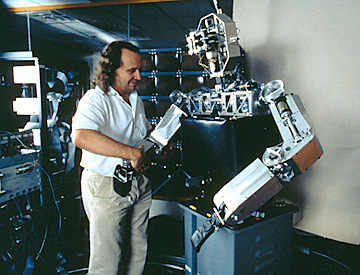
\includegraphics[height=5cm]{brooks_and_cog.jpg}}
    \hfil
     \subfloat[][Rodney Brooks and the Cog humanoid]{\label{}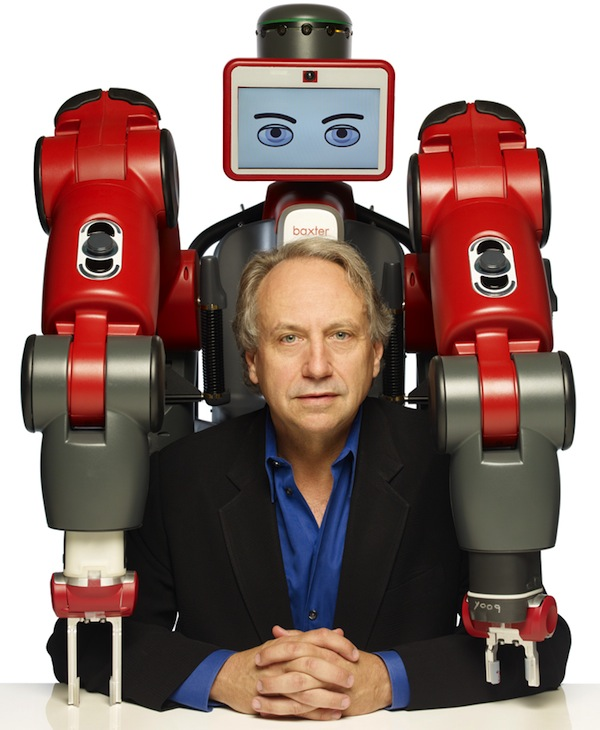
\includegraphics[height=5cm]{brooks_and_baxter.jpg}}\\
    \subfloat[][Cynthia Breazeal with Kismet]{\label{}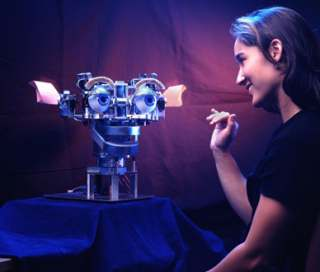
\includegraphics[height=5cm]{breazeal_kismet.jpg}}
    \hfil
    \subfloat[][Cynthia Breazeal with Kismet]{\label{}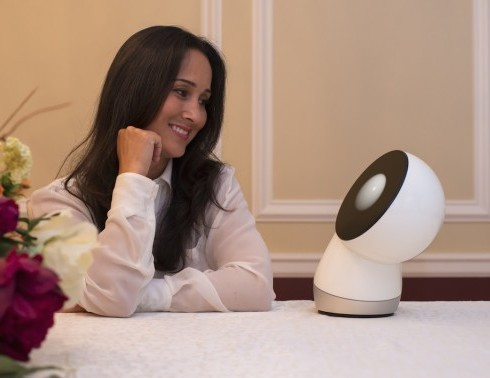
\includegraphics[height=5cm]{breazeal_and_jibo.jpg}}
    \caption{The Cog project was about the use of computer and robotic technology to better understand and emulate human intelligence.}
    \label{}
\end{figure}


\section{Mediation} % (fold)
Les astrophycisiens ont compri l'interet de la mediation, ils utilisent des artistes pour faire passer des concepts fondamentaux et n'ont plus à justifier d'un interet utilitaire, au moins à court terme, lié à leur recherche.
En robotique c'est pas le cas, nous sommes en permanance en train de justifier notre travail par rapport à une portée utilitaire à court terme comme l'assistance à la personne ou pire des applications militaires.

Si effectivement la robotique peut apporter certaines avancées technologiques dans ces domaines, il est dommage de devoir s'en justifier afin d'obtenir des fonds de recherche. Comme la physique, la robotique pose des questions fondamentales qui sont en soit très interessantes et devrait justifier à elles seules qu'on y accorde du credit.

Si on peut se cacher derriere le fait que les gens ne peuvent comprendre, on peut aussi remettre en cause les scientifique qui n'essaye pas de transmettre ces idées. Des collaborations artistiques peuvent être une piste de travail afin d'éduquer le public à ces questions fondamentales. Les artistes sont bien plus pertinents lorsqu'il s'agit de faire passer des idées, des concepts purs.

Rendre Poppy accessible aux artistes c'est aussi participer à cette mediation scientifique en donnant aux artistes un outil adapté avec lequel ils peuvent travailler et modifier. Si Poppy est encore un peu compliqué, l'interaction avec les fablabs peut être une solution. Les Poppy appartenant aux fablab, il pourrait être le pont entre l'artiste et le scientifique, apportant les competences techniques necessaires (programmation, réparation, formation, etc...) afin d'aider les artistes dans leur travaux. Tandis que les scientifiques auraient une discussion plus conceptuel.

\section{De nouveaux outils de publication scientifique} % (fold)

Une autre chose que l'on pourrait voler à l'art est la diversité des mediums utilisés.

En science nous utilisons depuis presque un siecle le papier en tant que publication scientifique. Il est le seul critère de notation scientifique et si quelque chose n'est pas publié alors il n'existe pas d'un point de vue scientifique. Tout le systeme d'évaluation, de partage et de frok est basé sur le papier.

A l'air du numérique et d'internet on peut raisonablement se poser la question si ce system est encore le plus adapté, surtout pourquoi ne pas avoir plusieur medium de communication scientifique. Est ce qu'une video youtube n'est pas une forme de publication, est ce que le fait de partager du code ou mieux une librairie n'est pas une forme de publication scientifique plus utile qu'un papier.

Aussi, comme dans le milieu artistique, certains personnes sont naturellement plus à l'aise avec certains medium (peinture, photos, installation, musique, ect ...), on peut raisonnablement penser que dans le milieu scientifique les même biais existent. Certains plus à l'aise avec la publication video, d'autres avec les graphiques, d'autres avec du code, du theatres,  etc ... Chaque outils étant plus ou moins adaptés en fonction de ce que l'on veut montrer.

La Science est un milieu de peer-review, ça ne tient qu'aux scientifiques d'accepter de reviewer d'autres medium que des papiers et de valider ça scientifiquement.


Les choses bougent un peu dans ce sens avec certains outils comme figshare ou open research platform. Cependant elles sont encore utilisées que part de petit thesard et pas par les grand ponte de la science.

La diversité est une base de la créativité

\section{Open science} % (fold)
Enfin un dernier point concerne la reproductabilité de la science. Une des valeurs fondamentales de la science et son universalité et ses valeurs de partages, dès lors il est etonnant de voir que dans les faits, tout est fait pour l'empecher. Le fait de noter la recherche d'un labo uniquement sur sa capacité à produire des papiers focus les effort de celui ci. De plus, aucune valeur ajouté n'est lié au fait que le code associé soit disponible, que les données soient disponibles etc ... Pourtant, il faut au moins compter un facteur 3 pour transformer un code qui marche pour un papier en un code qui est accessible et disponible pour être testé ailleurs, base de la science ...


Finalement, une quantité enorme de temps humain est gaché pour refaire ce qui a dejà était fait de multiple fois. C'est là où la science devrait s'inspirer du modèle open source du developpment logiciel. Il n'y a pas de raison que tout le monde fasse sont systeme de trie de liste alors que c'est normalement assez abstrait. Mettons tous au même endroit et developpons un bon code de trie de liste une fois pour toute.

Laissons les chercheurs passer du temps sur la recherche plutôt que le developpement. Le seul moyen c'est que les chercheurs partagent le materiel associé à leur recherche. Pour le moment seul les scientifiques engagés dans cette politique le font, au detriment de leur carriere car ça n'a aucune valeur académique. Il faudrait que ce soit reconnu comme étant effectivement une publication de qualité pour que ça plus adopté.
Ici encore, c'est du peer review, ça ne depend que des scientifiques d'accepter ou non des papiers qui ne mettent pas tout en place pour assurer la diffusion et la reproductabilité des resultats.


Encore une fois, on va dire que certain setup sont très compliqués à diffuser, cependant on peut maintenant s'appuyer sur le réseau des fablab. Il est justifier qu'un labo paye pour obtenir du materiel hardware, cet argent peut être utilisé pour payer un fablab afin qu'il reproduise le setup. Il y a des hacker space, des biospace et des maker space.





